\documentclass[12pt, letterpaper]{article}
\usepackage[margin=2cm]{geometry}
\usepackage{fourier}
\usepackage[T1]{fontenc}
\usepackage[utf8]{inputenc}
\usepackage{amsmath}
\usepackage{placeins}
\usepackage{bookmark}
\usepackage{hyperref}
\usepackage{booktabs}
\usepackage{textcomp}
\usepackage{graphicx}
\usepackage{wrapfig}
\usepackage{parskip}
\usepackage{epstopdf}
\usepackage[sorting=none,style=ieee]{biblatex}
\DeclareUnicodeCharacter{2009}{\,}
\setcounter{secnumdepth}{-\maxdimen}

\title{cuTimeWarp: Accelerating Soft Dynamic Time Warping on GPU}

\author{Alex Kyllo \and Afrooz Rahmati}

\addbibresource{cuTimeWarp.bib}

\begin{document}

\maketitle

\begin{abstract}

This report explores techniques for optimizing the computation of Soft Dynamic
Time Warping, a differentiable sequence dissimilarity measure, on graphics
processing units (GPU), for the purpose of enabling high-performance machine
learning on time series datasets.

\end{abstract}

\section{Introduction}

Time series machine learning is a research area with countless useful
applications such as recognizing sounds and gestures. Clustering or classifying
large time series datasets is challenging partly because of the need to define a
measure of dissimilarity between any two given time series. Furthermore,
practical applications require finding common structure in time series despite
different speeds or phases; for example, a word means the same whether spoken
quickly or slowly. Another requirement for machine learning tasks is that the
dissimilarity measure must be differentiable so that its gradient can be used as
to minimize it as a loss function to find the best fit model. Finally, the
measure must be efficient to calculate, because it will be calculated repeatedly
many times during model fitting. To this end we will explore GPU acceleration of
Soft Dynamic Time Warping (Soft-DTW) \cite{cuturi_soft-dtw_2018}, a
differentiable sequence dissimilarity measure, to enable high performance time
series machine learning.

\subsection{Background}

\subsubsection{Time series data}

Time series data generally refers to data containing quantitative measurements
collected from the same subject or process at multiple points in time, and it
exhibits several peculiarities in comparison to time-independent data.  Time
series data can exhibit autocorrelation, meaning that the value at any point in
time can exhibit correlation to the value at a previous point in time, with some
delay or \emph{lag} in between. Time series data can also exhibit
\emph{seasonality} or cyclical patterns as well as \emph{trend} which is a
tendency for the average value (over some rolling time window) to increase or
decrease as a function of time. Due to these characteristics, time series data
does not conform to the I.I.D. (independent and identically distributed)
assumption that typically applies in the study of random variables, and
therefore it requires special techniques for analysis and modeling.

Time series data can be either univariate or multivariate. For example, a set of
electrocardiogram (ECG) measurements has a single variable (heart voltage)
collected over time, but if the dataset also included the patient's blood
pressure and oxygen levels measured at each time point, that would constitute a
multivariate time series, and correlations between the different variables could
be studied in addition to the autocorrelation within each of the variables.

\subsubsection{Time series distance and dissimilarity measures}

A fundamental capability that enables analysis of and learning from data is the
ability to quantify a measure of distance or dissimilarity between observations.
For time-independent data, (TODO)

There are multiple valid ways to compute a measure of dissimliarity between two
time series; the simplest is Euclidean distance, which is the square root of the
sum of squared pairwise differences between two time series $x$ and $y$, each of
length $n$ (equation \ref{euclid}).

\begin{equation} \label{euclid}
d(x, y) = \sqrt{\sum_{t=1}^{n}(x_t-y_t)^2}
\end{equation}

The drawback of Euclidean distance in time series applications is that two
structurally similar time series will produce a large distance if they are
different speeds or out of phase (TODO: Add a figure to illustrate this).

\subsubsection{Dynamic Time Warping}

Dynamic Time Warping (DTW) was devised in the 1960s as an alternative time
series dissimilarity measure to address this shortcoming. (TODO: find a
historical citation). DTW is a nonlinear mapping of from each point in one time
series to the nearest point in a second time series. While DTW is technically
not considered a ``distance'' because it does not conform to the triangle
inequality, and therefore we refer to it as a ``dissimilarity'' instead, it can
be used in place of Euclidean distance or other distance measures for many
applications of time series data.

The purpose of (DTW) is to perform a transformation
function that wrap the time to align two time series. Preferably we tend this
alignment to be optimum and satisfy our
requirements.\cite{deriso_general_nodate}

DTW is a widely used tool employed in many areas of science, including biology,
technology, economics, and finance. It calculates the practical distance between
two signals typically by taking the distance between them when one is time
warped, or it can be the minimum wrapping required to align signals with each
other by applying some sort of fidelity.  Dynamic time wrapping can be used to
identify hidden pattern or searching within signals databases to find the
matching one.\cite{keogh_derivative_2001} it is utilized in machine learning
platforms that depends on signals like clustering, regression, and
classification.

The basic algorithm for DTW is to use Bellman’s recursion, a dynamic programming
technique, to find the lowest-cost path diagonally across a pairwise distance
matrix. The computation cost for this approach is quadratic ($O(mn)$) for time
series vectors of length m and n \cite{cuturi_soft-dtw_2018}. The formula for
the DTW between time series x and y is given by equation \ref{dtw}.
(TODO: explain the algorithm in more detail and provide a visualization)

\begin{equation} \label{dtw}
DTW(x,y) = min_{\pi}\sqrt{\sum_{(i,j)\in\pi}d(x_{i},y_{j})^2}
\end{equation}

Where $d(x_i,y_j)^2$ is the cost function, typically pairwise squared Euclidean
distance. The loss function for DTW is not differentiable due to the min
operation within the formula; a small change in the input time series may result
in zero change in the path cost. However, we can create a differentiable version
called Soft-DTW by replacing the min function with a soft-min function
(equation \ref{softdtw}) \cite{cuturi_soft-dtw_2018}.

\begin{equation} \label{softdtw}
\text{soft-min}_\gamma(a_1,...,a_n) = -\gamma log\sum_{i}e^{-a_i/\gamma}
\end{equation}

Hence, Soft-DTW is parameterized by the smoothing constant gamma, which becomes
a tunable hyperparameter in machine learning model training applications.

A common technique in machine learning with Soft-DTW is the computation of
barycenters, which are centroids within the space of a set of time series. The
differentiability of Soft-DTW allows for barycenter finding via gradient
descent, and then new observations can be classified by finding the nearest
barycenter. Sequence prediction and generation of is also possible using
recurrent neural networks with Soft-DTW as a loss function
\cite{cuturi_soft-dtw_2018}.

(TODO: Explain process of barycenter finding with gradient descent on softdtw
loss)

Prior to computing the Soft-DTW dissimilarity between any two time series, each
time series should be \emph{z-normalized}, that is, scaled so that its mean is
equal to 0 and its standard deviation is equal to 1, to remove the problem of
``wandering baselines'' or ``drift'' in the measurements, as illustrated in
\cite{rakthanmanon_addressing_2013} with an ECG classifier that yields incorrect
results on un-normalized data due to drift that ``may be caused by patient
movement, dirty lead wires/electrodes, loose electrodes, and so on,'' and which
``does not have any medical significance.'' Z-normalization also tends to make
the iterative process of minimizing the cost function through gradient descent
or quasi-Newtonian methods more efficient because its hyperplane is not
disproportionately stretched in any one dimension, so the step size in any
direction is the same relative to the scale of that dimension. (TODO: explain
this better, find a citation)

\subsubsection{Parallelizing DTW}

A naive, sequential implementation of DTW would involve a nested loop to iterate
over each row/column of the cost matrix to update its cost based on the three
neighboring cells' costs, hence the $O(n^2)$ time complexity. But because each
cell has a data dependency on the three cells to the top, left, and top-left,
there is no dependency between cells that are on the same antidiagonal of
the matrix, therefore computation of these cells can be handled by parallel
threads. One thread computes the upper-leftmost cell, then two threads compute
the next antidiagonal, then three threads compute the next, and so on.

\subsection{Related Work}

Utilizing indexing to construct lower bounds on warping distance is an
optimization technique for speeding up nearest neighbor search via early removal
of poor candidates \cite{keogh_exact_2002}. Shen and Chi (2021) proposes an
optimization of nearest neighbor search of multivariate time series, leveraging
the triangle inequality and quantization-based point clustering to restrict the
search \cite{shen_tc-dtw_2021}.

Xiao et al (2013) introduced a prefix computation technique for transforming the
diagonal data dependence to improve parallel computation of the cost matrix on
GPU \cite{xiao_parallelizing_2013}. Zhu et al (2018) demonstrates a method of
optimizing  memory access by taking advantage of the diagonal data dependency to
rearrange the matrix so that elements on the same diagonal are stored
contiguously \cite{zhu_developing_2018}. A prior implementation of Soft-DTW on
CUDA using PyTorch and Numba is capable of 100x performance improvement over the
original Soft-DTW Cython code, but is limited to sequence lengths of 1024 (CUDA
max block size) and leaves many opportunities for further CUDA optimizations
such as the use of shared memory \cite{maghoumi_pytorch-softdtw-cuda_2021}. A
2015 paper describes a tiling approach called \emph{PeerWave}, which utilizes
direct synchronization between neighboring streaming multiprocessors (SMs) to
handle the inter-tile data dependency without atomic operations, locks, or other
global barriers, leading to improved load balance and scaling properties
\cite{belviranli_peerwave_2015}.

In our project we will focus on this area of opportunity, optimizing matrix
structure and memory access patterns to maximize parallelism and minimize memory
latency in the computation of the warping path matrix.

\section{Methods}

To evaluate various performance optimizations on the Soft-DTW computation, we
implemented a C++ and CUDA library called cuTimeWarp, which includes functions
for computing the SoftDTW on CPU and GPU.

Given a set of many multivariate time series of the same length and number of
variables, we can compute the Soft-DTW distance between every time series and
every other time series in the set by computing, in parallel for each pair, a
pairwise squared Euclidian matrix, then applying the Soft-DTW calculation on the
distance matrix. This computation, however, also has an $O(n^2)$ complexity and
can potentially even take longer than the DTW computation itself. For univariate
time series, we can save this cost by computing the DTW cost matrix on the two
input time series directly, computing the absolute distance between each pair of
values from the two time series within the nested loop of the DTW procedure.

\subsection{Optimization Techniques}

\subsubsection{Wavefront Tiling}
Wavefront parallelism is one of the useful methods to overcome the dependencies of nested loops 
by multiple processing units. The idea is to re-order the loop iterations in such a way that 
form diagonal wave and each wave can be computed in parallel. Barriers will be utilized to control 
the data dependencies among consecutive waves. Elements inside the wave grouped together using tiled 
technique to enhance data locality and performance. This methodology presents a second degree of parallelism 
where tiles can be computed in parallel by separating with a global variable.

GPU and specifically CUDA can accelerate the process of wavefront. Each tile assigns 
to a block to be process in parallel by SM. On the other hand, the iteration along diagonals within a tile are also
pluralized. In order to enforce the dependencies, the global barriers used among the tiles and within every tiles.\cite{belviranli_peerwave_2015}     

In our Soft DTW implementation, we utilized the wavefront technique to manage the dependencies of neighboring cells for 
computing the minimum warp path. In our algorithm this value depends on the minimum cost of the upper, 
left and upper-left diagonal cell cost. Figure \ref{DTW_dependency} show this dependencies clearly.Each D(i,j) depends on the up, left and up-left neighbor cost. 

\begin{figure}[htbp]
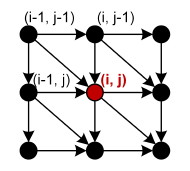
\includegraphics[height=2in]{img/tiling_dependencies.png}
\centering
\caption{computation dependencies for DTW.}
\label{DTW_dependency}
\end{figure}

Wavefront process split to three major steps:

\begin{itemize}
  \item Populating the dependencies managing by loop. In this step, we keep the global variable WaveId to sperate the process of waves. Wavelength is increasing one by one on each loop iterations until reaching the total number of tiles. The primary kernel softdtw global tiled called with the wavelength number of blocks and thread size of tile width.
  \item In this kernel, the row and column index for each tile is calculating and passing as a global variable to the corresponding kernel for the tiles’ computation.
  \item The third step is the main kernel to process inter-tiles in parallel. Shared memory employed to keep the tile within the cache and improve the overall performance. As we mentioned earlier, we need to calculate the soft-min for the dependent cells. Therefore, the soft-min calculated for the up, left and diagonal upper left index.(equation \ref{dependencies})
\end{itemize}

\begin{equation} \label{dependencies}
  D (i,j) = Soft-min
  \begin{cases}
        D(i-1,j) \\
        D(i,j-1)\\
        D(i-1,j-1)   
  \end{cases}
\end{equation}
Drawbacks:
Due to the usage of global barriers, there would be lower utilization for the GPU. 
Fewer threads would be available at the beginning and at the end of each tiles process. 
Also, less tiles are accessible toward the beginning and end of wave iterations. 
Therefore, device SM remain idle during the initiation and end of the process. 

\subsubsection{Diagonal-major layout}

Because the data dependency structure of the DTW algorithm results in elements
of the distance and cost matrices on the same antidiagonal being processed in
parallel, storing these matrices in row-major or column major order will cause a
performance impact from cache misses and non-coalesced accesses to global
memory.

If the data is first rearranged into an antidiagonal-major layout, then at each
iteration of the wavefront loop, processor threads will make coalesced accesses
to data elements that are laid out contiguously in memory.

\subsubsection{Shared memory stencil computation}

As the program iterates diagonally across the distance matrix to find the
optimal warping path, each cell in the path utilizes the previously computed
results of three previous neighboring cells; if the iteration is visualized as
proceeding from the upper left to the lower right corner of the matrix, the cost
value in each cell depends on the (soft) minimmum of the costs in the cell
above, the cell to the left, and the cell to the diagonal upper-left, which were
computed in the previous two iterations (Figure \ref{cost_deps}). If the cost
matrix \verb|R| resides in global memory, then non-contiguous accesses to
\verb|R[i-1][j]|, \verb|R[i][j-1]| and \verb|R[i-1][j-1]| will result in cache
misses, incurring a significant performance cost. Since each element of \verb|R|
will be referenced up to three times in the computation of dependent cells,
these cache misses can be avoided via a stencil computation using shared memory
in CUDA. The stencil serves as a cache for the current and previous two
diagonals; once a diagonal is no longer in use, its elements are written back to
the cost matrix \verb|R| in device global memory.

\begin{figure}[htbp]
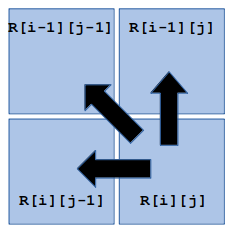
\includegraphics[height=2in]{img/cost_dependencies.png}
\centering
\caption{Data dependency direction between cells of the cost matrix.
Each cell's cost computation depends on the costs of the three adjacent cells
above, to the left, and to the upper-left.}
\label{cost_deps}
\end{figure}

\FloatBarrier
The algorithm can be modified to use shared memory as follows:

\begin{verbatim}
D is a squared euclidean distance matrix of two time series
R is a cost matrix initialized to positive infinity except for R[0, 0] = 0
for each anti-diagonal of R starting from R[0, 0]
    if the current thread index < length of the current anti-diagonal
        copy R[i][j] from global memory into the stencil array
        read R[i-1][j], R[i][j-1] and R[i-1][j-1] from the stencil array
        compute cost as softmin(R[i-1][j], R[i][j-1], R[i-1][j-1]) + D[i-1][j-1]
        write the cost back to the stencil
        copy the cost in R[i-1][j-1] from the stencil back to global memory
\end{verbatim}
\FloatBarrier

\subsubsection{Sakoe-Chiba bands}

Sakoe-Chiba bands, proposed by Sakoe and Chiba in their 1978 paper "Dynamic
programming algorithm optimization for spoken word recognition," introduce a
"slope constraint" to the warping path to limit the maximum allowed warping
distance beyond which a pair will not be considered in the optimal path
calculation \cite{sakoe_dynamic_1978}. Pruning the search space by removing some
of the extreme diagonals from consideration yields an approximation of the
optimal warping path that can be calculated in sub-quadratic time.

This optimization is simple to implement for square matrices (i.e. DTW on time
series of equal length) by checking that the absolute difference between the
loop counter variables \verb|i| and \verb|j| does not exceed a fixed bandwidth
threshold value (Figure \ref{sakoe_chiba}). For rectangular matrices, since the
leading diagonal does not end at the lower right corner, the implementation must
be slightly modified to ensure that the counter variable along the longer of the
two dimensions stays within a defined radius. Either way the result is a
diagonal band matrix.

In a parallel programming environment such as CUDA, this optimization can also
allow for the computation of the warping path using fewer threads, as threads
assigned to cost matrix cells outside the band would go unused. Space savings
can also be obtained if the bandwidth is known in advance, by storing the
distance matrix and cost matrix in band storage format, omitting the zeroes
in the corners.

While this technique produces only an approximation of the optimal path, in
practice it has been shown to improve task performance by preventing
pathological alignments where a very small portion of one time series maps onto
a large portion of the other \cite{keogh_exact_2002}. The width of the band
can be a tunable hyperparameter for time series classification tasks.

\begin{figure}[htbp]
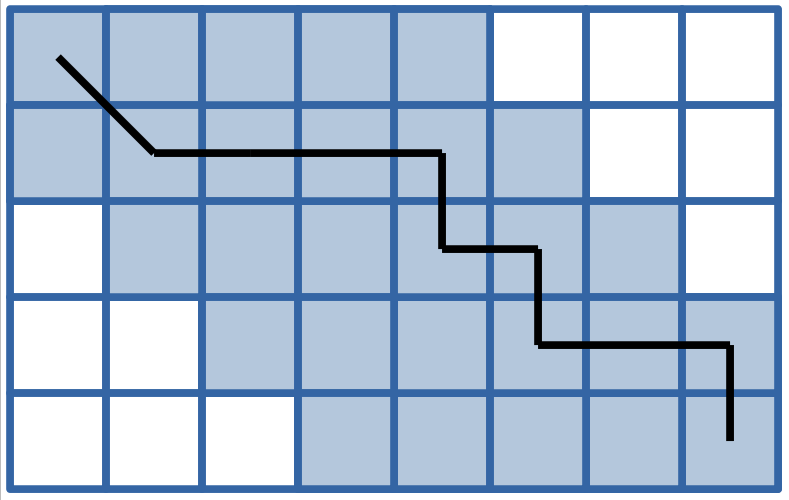
\includegraphics[height=2in]{img/sakoe_chiba.png}
\centering
\caption{Illustration of one possible optimal DTW path for a length 5 series and
a length 8 series with Sakoe-Chiba band radius = 1.}
\label{sakoe_chiba}
\end{figure}


\subsection{Test Data}

For performance testing we selected datasets from the UCR Time Series Archive
\cite{dau_ucr_2019} and the UEA Multivariate Time Series Classification Archive
\cite{bagnall_uea_2018}.

\section{Results}

\section{Discussion}

\section{Future Work}

Our library provides CUDA kernels and C++ wrappers for computing pairwise
Soft-DTW dissimilarity measures as well their gradients in parallel. Potential
future work includes integrating this library with an optimization library that
can iteratively minimize Soft-DTW cost to find barycenters among a set of time
series, to assemble a nearest centroid classification system. Another area of
potential is writing Python bindings to expose the Soft-DTW loss and gradient
functions to deep learning frameworks such as TensorFlow or PyTorch, to enable
the use of Soft-DTW loss as a training objective for recurrent neural networks.
This will facilitate tasks such as classifying, predicting and generating sounds,
gestures, and sensor data under the dynamic time warping geometry.

\printbibliography[]
\end{document}
